%% Technical Report for the work on the AI-DSL over the period of
%% March to May 2021.

\documentclass[]{report}
\usepackage{url}
\usepackage{minted}
\usepackage[textsize=footnotesize]{todonotes}
\newcommand{\kabir}[2][]{\todo[color=yellow,author=kabir, #1]{#2}}
\newcommand{\nil}[2][]{\todo[color=purple,author=nil, #1]{#2}}
\usepackage[hyperindex,breaklinks]{hyperref}
\usepackage{breakurl}
\usepackage{listings}
\lstset{basicstyle=\ttfamily\footnotesize,breaklines=false,frame=single}
\usepackage{float}
\restylefloat{table}
\usepackage{longtable}
\usepackage{graphicx}
\usepackage[font=small,labelfont=bf]{caption}
\usepackage[skip=0pt]{subcaption}
\usepackage{circledsteps}

\begin{document}

\title{AI-DSL Technical Report (February to May 2021)}
\author{Nil Geisweiller, Kabir Veitas, Eman Shemsu Asfaw, Samuel Roberti}
\maketitle

\begin{abstract}
This document is a technical report of a work done between February
and May 2021, based on the \emph{AI-DSL
Proposal}~\cite{GoertzelGeisweillerBlog} published as a blogpost on
the SingularityNET website in December 2020.  It is the first
iteration of a larger endeavor to create a system that enables
autonomous interoperability between AI services over the network, more
specifically over the SingularityNET-on-Cardano network.  It presents
in detail what has been accomplished so far as well as future plans
for the continuation of that endeavor.
\end{abstract}

\tableofcontents

\chapter{Introduction}
\section{Autonomous Interoperability of AI Services}
Among the wonders that the blockchain technology enables is the
possibility to programmatically exchange values and services between
parties.  In the context of AI services it becomes especially relevant
given the inherent complexity and decomposability of such systems.
Moreover, the abundance of AI algorithms available on the Internet
makes it that often creating a new AI solution consists of connecting
together existing AI algorithms.  For instance building a system to
discover new drugs may consist of
\begin{enumerate}
\item a reasoner to extract background knowledge from biological
  databases,
\item a principal component analyzer to discover abstractions,
\item a feature selector to discard irrelevant information,
\item a learner to generate predictive models relating selected
  features and drug efficacy.
\end{enumerate}
The task of composing such AI algorithms is, in most cases, done by
humans and, as any AI practitioner knows, is tedious and time
consuming.  Not just the composition of the whole but also the search
and the understanding required to find the parts.  Facilitating and
ultimately automating such process is the goal of the \emph{Artificial
Intelligence Domain Specific Language}, or \emph{AI-DSL} for short.

Another important aspect is the management of resources, both
financial and computational (CPUs, GPUs, etc).  The AI-DSL is also
intended to incorporate descriptions of such computational
requirements as well as measures of expected result quality.

Finally, as described in the blogpost, the current plan is to have
such system rely on Dependent Types~\cite{Altenkirch05whydependent} to
express and validate the specifications of the AI services, including
cost, quality and their relationships thereof.  The reason Dependent
Types have been chosen is because they are geared toward program
specification checking and program generation, which in our case comes
close to AI services verification and combination if one sees AI
services as functions.  More specifically Idris has been chosen as our
initial Dependently Typed Language (DTL) candidate, due to its
efficiency and the fact that is has been primarily designed to verify
and generate actual running programs as opposed to
proofs~\footnote{Programs are equivalent to proofs according to the
Curry-Howard correspondence but some representations are more amenable
to running actual programs than others}.

\section{Objectives and accomplishments}
For that first iteration the goals were to
\begin{enumerate}
\item Experiment with matching and retrieval of AI services using
  Idris~\cite{Idris}, a Dependently Typed Language (DTL)~\cite{DTL},
  equipped with a powerful type system to express function
  specifications.  That work is described in
  Chapter~\ref{chap:aidsl_registry}.
\item Start building an AI ontology to ultimately provide a rich and
  extendable vocabulary for the AI-DSL.  That work is described in
  Chapter~\ref{chap:aidsl_ontology}.
\item Start building the AI-DSL itself, from its syntax to its
  semantics.  Exploratory work on that is described in
  Chapter~\ref{chap:soft_eng_strat}.
\item Integrate all the above into a holistic prototype, running on a
  real world test case of AI service assemblage, in real conditions,
  that is ideally on the SingularityNET-on-Cardano network.
  Preparatory work on that is described in
  Section~\ref{sec:net_ai_future_work}.
\end{enumerate}
All the objectives except the last one have been accomplished at
least to some degree.  The last, and the most ambitious, objective had
to be postponed for the next iteration due to its complexity.

\section{Related work}
\label{sec:related_work}
To the best of our knowledge there is no existing work on creating
such AI-DSL system to enable autonomous AI services interoperability
using Dependent Types, let alone running on a blockchain.  There are
however attempts using related methodologies, usually involving
ontologies with more or less explicit forms of reasoning, outside of
the context of the blockchain technology.

We are collecting a body of literature in a github
issue~\cite{AIDSLRelatedWork} serving as a living document and being
regularly updated with such related work.  We will not describe the
entire body here due to its volume (over 70 references at the time of
writing) and the fact that we are still in the process of reviewing
it.  Here is however the most relevant work we have encountered so
far.

The most recent and also most relevant work we have found is the
Function Ontology~\cite{FunctionOntology, DeMeester2020}. Its goal is
to define a standard for describing, both formally and informally,
functions, their references to implementations, as well as developing
tools for retrieving and executing them, remotely or locally.  To the
best of our knowledge it does not make use of dependent types or
blockchain technology, however there is a lot of potential for reuse.
More investigation will be conducted to precisely determine to what
extent.

Still relevant work with potential for reuse if only conceptual is
described below.  Let us start with the multi-agent system (MAS)
field. In~\cite{Brazier1995} the authors describe a use case of a
system called DESIRE, to formally define inputs and outputs of agents
and their control flows.  The logic seems somewhat limited but their
goals align with ours.  In~\cite{Bourahla20055} an extension of
Computation Tree Logic (CTL) called multi-modal branching-time logic
is defined to apply model checking on collections of agent given their
description in some abstract programming language.  It's not clear the
specification language they use is very convenient and the model
checking methodology is open-ended enough, but nevertheless the work
is solid and relevant.  In~\cite{Desouky2007} is described an
architecture for distributed multi-agent intelligent system.  The
description of the architecture is high level but the authors mention
Agent Communication Language (ACL) standards~\cite{Labrou99thecurrent}
such as FIPA-ACL~\cite{FIPAACL}, used to communicate agents requests
to each other.  In the ontology field we have found the following
papers.  In~\cite{Gruber_anontology} the authors introduce an ontology
called EngMath for representing mathematical concepts useful for
engineering, including quantity units, equations and more in
KIF~\cite{KIF} to be used in SHADE~\cite{Gruber92towarda} a system for
collaborative intelligent agents.  It is rather old and it seems
development has halted, but could nevertheless be interesting to learn
more about.  OpenMath~\cite{Abbot1995} is another old, but still
maintained, ontology about mathematics.  More recent mathematical
ontologies worth mentioning are OntoMath~\cite{Elizarov2017} and
OntoMathPRO~\cite{nevzorova2014ontomathpro}, they seem rather high
level but could still be useful.  Broadening the scope,
\cite{Roelofs2020} is focused on validating the consistency of
ontologies.  Relatedly, in~\cite{Witherell2009}, a tool for analyzing
and propagating changes across overlapping ontologies according to
predefined inference rules, called FIDOE, is introduced.  The authors
mention standards such as SUMO~\cite{pease_standard_2009} and
SWRL~\cite{SWRL} as well.  Such work could be relevant towards the
goal of facilitating the decentralization of the AI-DSL and its
ontology.

\chapter{AI-DSL Registry}
\label{chap:aidsl_registry}

In this chapter we describe a prototype of an AI-DSL registry, a
service in charge of storing AI service specifications and returning
matching AI services upon request, given a specification to fulfill.
In Section \ref{sec:realized_function} we describe experiments for
implementing the \texttt{RealizedAttributes} and
\texttt{RealizedFunction} data structures described
in~\cite{GoertzelGeisweillerBlog} used for capturing financial,
computation costs, as well as measures of expected result quality.  In
Section \ref{sec:network_idris_ai_services} we describe the implementation
of a network of trivially simple AI services implemented in Idris, and
use the Idris compiler to type check if they can properly connect to each
other.  Finally, in Section \ref{sec:dependently_typed_registry} we describe the
implementation of an AI-DSL Registry prototype, as a proof-of-concept
for querying AI services based on their dependently typed
specifications.

\section{Realized Function}
\label{sec:realized_function}

\subsection{Description}

The \texttt{RealizedFunction} data structure, as introduced
in~\cite{GoertzelGeisweillerBlog}, is a wrapper around a regular
function to integrate aspects of its specifications pertaining to its
execution on real physical substrates as opposed to just its
algorithmic properties.  For instance it contains descriptions of
costs (financial, computational, etc) and performances (quality, etc)
captured in the \texttt{RealizedAttributes} data structure, as
introduced in~\cite{GoertzelGeisweillerBlog} as well.

For that iteration we have implemented a simple version of
\texttt{RealizedFunction} and \texttt{RealizedAttributes} in
Idris2~\cite{Idris}.  The \texttt{RealizedAttributes} data structure
contains
\begin{itemize}
\item \texttt{Costs}: as a triple of three constants,
  \texttt{financial}, \texttt{temporal} and \texttt{computational},
\item \texttt{Quality}: as a single \texttt{quality} value.
\end{itemize}
as well as an example of compositional law,
\texttt{add\_costs\_min\_quality}, where costs are additive and
quality is infimum-itive.  Below is a small snippet of that code to
give an idea of how it looks like

\begin{minted}[mathescape]{idris}
record RealizedAttributes where
  constructor MkRealizedAttributes
  costs : Costs
  quality : Quality
\end{minted}

\begin{minted}[mathescape]{idris}
add_costs_min_quality : RealizedAttributes ->
                        RealizedAttributes ->
                        RealizedAttributes
add_costs_min_quality f_attrs g_attrs = fg_attrs where
  fg_attrs : RealizedAttributes
  fg_attrs = MkRealizedAttributes (add_costs f_attrs.costs g_attrs.costs)
                                  (min f_attrs.quality g_attrs.quality)
\end{minted}
The full implementation can be found in
\href{https://github.com/singnet/ai-dsl/blob/master/experimental/realized-function/RealizedAttributes.idr}{\texttt{RealizedAttributes.idr}},
under the
\href{https://github.com/singnet/ai-dsl/blob/master/experimental/realized-function/}{\texttt{experimental/realized-function/}}
folder of the \href{https://github.com/singnet/ai-dsl/}{AI-DSL
  repository}~\cite{AIDSLRepo}.\\

Then we have implemented \texttt{RealizedFunction} that essentially
attaches a \texttt{RealizedAttributes} instance to a function.  In
addition we have implemented a composition (as in function
composition) operating on \texttt{RealizedFunction} instead of
regular function, making use of that compositional law above.
Likewise below is a snippet of that code

\begin{minted}[mathescape]{idris}
data RealizedFunction : (t : Type) -> (attrs : RealizedAttributes) -> Type where
  MkRealizedFunction : (f : t) -> (attrs : RealizedAttributes) ->
                       RealizedFunction t attrs
\end{minted}

\begin{minted}[mathescape]{idris}
compose : {a : Type} -> {b : Type} -> {c : Type} ->
          (RealizedFunction (b -> c) g_attrs) ->
          (RealizedFunction (a -> b) f_attrs) ->
          (RealizedFunction (a -> c) (add_costs_min_quality f_attrs g_attrs))
compose (MkRealizedFunction g g_attrs) (MkRealizedFunction f f_attrs) =
  MkRealizedFunction (g . f) (add_costs_min_quality f_attrs g_attrs)
\end{minted}
The full implementation can be found in
\href{https://github.com/singnet/ai-dsl/blob/master/experimental/realized-function/RealizedFunction.idr}{\texttt{RealizedFunction.idr}}
under the same folder.

Given such data structure we used the Idris compiler to type check if
the realized attributes of realized functions, i.e. AI services,
composed from other realized functions would follow the defined
compositional law, here \texttt{add\_costs\_min\_quality}.  That is given
for instance the realized attributes of an incrementer function
\begin{minted}[mathescape]{idris}
incrementer_attrs = MkRealizedAttributes (MkCosts 100 10 1) 1
\end{minted}
and a twicer function
\begin{minted}[mathescape]{idris}
twicer_attrs = MkRealizedAttributes (MkCosts 200 20 2) 0.9
\end{minted}
the realized attributes of their compositions must be
\begin{minted}[mathescape]{idris}
rlz_compo1_attrs = MkRealizedAttributes (MkCosts 300 30 3) 0.9
\end{minted}
otherwise Idris detects a type error.

\subsection{Objectives and achievements}

The objectives of this work was to see if Idris2 was able to type
check that the realized attributes of composed realized functions
followed the defined compositional law.  We have found that Idris2 is
not only able to do that, but to our surprise does it considerably
faster that Idris1 (instantaneous instead of seconds to minutes), by
bypassing induction on numbers and using efficient function-driven
rewriting on the realized attributes instead.

That experiment can be found in
\href{https://github.com/singnet/ai-dsl/blob/master/experimental/realized-function/RealizedFunction-test.idr}{\texttt{RealizedFunction-test.idr}},
under the
\href{https://github.com/singnet/ai-dsl/blob/master/experimental/realized-function/}{\texttt{experimental/realized-function/}}
folder of the \href{https://github.com/singnet/ai-dsl/}{AI-DSL
  repository}~\cite{AIDSLRepo}.

An improvement of that work is also described in Section
\ref{sec:service_composition_in_idris2}.

\subsection{Future work}

Experimenting with constants as realized attributes was the first step
in our investigation.  The subsequent steps will be to replace
constants by functions, probability distributions and other
sophisticated ways to represent costs and quality.

\section{Network of Idris AI services}
\label{sec:network_idris_ai_services}

\subsection{Description}

In this work we have implemented a small network of trivially simple
AI services, with the objective of testing if the Idris compiler could
be used to type check the validity of their connections. Three primary
services were implemented
\begin{enumerate}
\item \texttt{incrementer}: increment an integer by 1
\item \texttt{twicer}: multiply an integer by 2
\item \texttt{halfer}: divide an integer by 2
\end{enumerate}
as well as composite services based on these primary services, such as
\begin{itemize}
\item \texttt{incrementer . halfer . twicer}
\end{itemize}
with the objective of testing that such compositions were properly
typed.  The networking part was implemented based on the
SingularityNET example service~\cite{SNETExampleService} mentioned in
the SingularityNET tutorial~\cite{SNETTutorial}.  The specifics of
that implementation are of little importance for that report and thus
are largely ignored.  The point was to try to be as close as possible
to real networking conditions.  For the part that matters to us we may
mention that communications between AI services are handled by
gRPC~\cite{gRPC}, which has some level of type checking by insuring
that the data being exchanged fulfill some type structures (list of
integers, union type of string and bool, etc) specified in Protocol
Buffers~\cite{Protobuf}.  Thus one may see the usage of Idris in that
context as adding an enhanced refined verification layer on top of
gRPC making use of the expressive power of dependent types.

\subsection{Objectives and achievements}

As mentioned above the objectives of such an experiment was to see how
the Idris compiler can be used to type check combinations of AI
services.  It was initially envisioned to make use of dependent types
by specifying that the \texttt{twicer} service outputs an even
integer, as opposed to any integer, and that the \texttt{halfer}
service only accepts an even integer as well.  The idea was to
prohibit certain combinations such as
\begin{itemize}
\item \texttt{halfer . incrementer . twicer}
\end{itemize}
Since the output of \texttt{incrementer . twicer} is provably odd,
\texttt{halfer} should refuse it and such combination should be
rejected.  This objective was not reached in this experiment, but was
reached in the experiments described in Sections
\ref{sec:dependently_typed_registry} and \ref{sec:dependent_pairs}.
The other objective was to type check that the compositions have
realized attributes corresponding to the compositional law implemented
in Section \ref{sec:realized_function}, which was fully achieved in
this experiment.  For instance by changing either the input/output
types, costs or quality of the following composition
\begin{minted}[mathescape]{idris}
-- Realized (twicer . incrementer).
rlz_compo1_attrs : RealizedAttributes
rlz_compo1_attrs = MkRealizedAttributes (MkCosts 300 30 3) 0.9
-- The following does not work because 301 /= 200+100
-- rlz_compo1_attrs = MkRealizedAttributes (MkCosts 301 30 3) 0.9
rlz_compo1 : RealizedFunction (Int -> Int) Compo1.rlz_compo1_attrs
rlz_compo1 = compose rlz_twicer rlz_incrementer
\end{minted}
defined in
\href{https://github.com/singnet/ai-dsl/blob/master/experimental/simple-idris-services/service/Compo1.idr}{\texttt{experimental/simple-idris-services/service/Compo1.idr}},
the corresponding service would raise a type checking error at start
up.  More details on the experiment and how to run it can be found in
the
\href{https://github.com/singnet/ai-dsl/blob/master/experimental/simple-idris-services/README.md}{\texttt{README.md}}
under the
\href{https://github.com/singnet/ai-dsl/blob/master/experimental/simple-idris-services/}{\texttt{experimental/simple-idris-services/service/}}
folder of the \href{https://github.com/singnet/ai-dsl/}{AI-DSL
  repository}~\cite{AIDSLRepo}.

Thus besides the fact that dependent types were ignore in that
experiment, the objectives were met.  See Section \ref{sec:dependently_typed_registry}
for a follow up experiment involving dependent types.

\subsection{Future work}
\label{sec:net_ai_future_work}
Such experiment was good to explore how Idris can be integrated to a
network of services.  What we need to do next is experiment with
actual AI algorithms, making full use of dependent types in their
specifications.  Such endeavor was actually attempted over the Fake
News Warning app described in Section
\ref{sec:domain_model_considerations}, but it was eventually concluded
to be too ambitious for that iteration and was postponed for the next.

To briefly recall here, the Fake News Warning app is an AI service
assemblage to estimate if the headline of an article is consistent
with its body.  Such assemblage is composed of
\begin{enumerate}
\item a few classifiers, each attempting to learn to recognize if the
  headline of an article is consistent with its body;
\item an aggregator combining the outputs of all classifiers into a
  single answer.
\end{enumerate}
So what we would like to achieve is to
\begin{enumerate}
\item formally specify the function of each AI service above (this
  will require to enrich the leaf ontology described in
  Section~\ref{sec:ontology_prototype} as well as the composition
  functions described in Sections~\ref{sec:realized_function} and
  \ref{sec:service_composition_in_idris2});
\item populate the AI-DSL registry described in
  Section~\ref{sec:dependently_typed_registry} with these formal
  specifications;
\item TODO
\end{enumerate}

 above likely ca categorical distributions over categories Towards
 that end we did however started to

An intermediary step, before moving to actual AI algorithms, is to
explore multi-facet specifications and their interactions with other
AI services.  That is, given AI services A, B and C, let's assume A's
output must satisfy a combination of properties, such as an integer
that is both even and within a certain interval.  Then B and C may
have need partial constraints to be fulfilled.  For instance B may
require an even integer, while C may require that integer to be within
a certain interval.  In other words both services B and C may take the
output of A as input but for different reasons.  It's obviously not
conceptual difficult to cast the output of A to match the input types
of B and C, however it is still something we need to explore with
Idris in its full generality.

Also, we obviously want to be able to reuse existing AI services and
write their specifications on top of them, as opposed to writing both
specification and code in Idris/AI-DSL.  To that end it was noted that
having a Protobuf to/from Idris/AI-DSL converter would be useful, so
that a developer can start from an existing AI service, specified in
Protobuf, and enriched it with dependent types in Idris/AI-DSL.  The
other way around could be useful as well to enable a developer to
implement AI services entirely in Idris/AI-DSL and expose their
Protobuf specification to the network.  Relatedly having directly an
implementation of gRPC for Idris/AI-DSL could be handy as well.

\section{Dependently Typed Registry}
\label{sec:dependently_typed_registry}

\subsection{Description}

One important goal of the AI-DSL is to have a system that can perform
autonomous matching and composition of AI services, so that provided
the specification of an AI, it should suffice to find it, complete it
or even entirely build it from scratch.  We have implemented an
\emph{AI-DSL Registry} proof-of-concept to start experimenting with
such functionality.

So far we have two versions in the
\href{https://github.com/singnet/ai-dsl/}{AI-DSL repository}, one
without dependent types support, under
\href{https://github.com/singnet/ai-dsl/blob/master/experimental/registry/}{\texttt{experimental/registry/}},
and a more recent one with dependent type support that can be found
under
\href{https://github.com/singnet/ai-dsl/blob/master/experimental/registry-dtl/}{\texttt{experimental/registry-dtl/}}.
We will focus our attention on the latter which is far more
interesting.\\

The AI-DSL registry (reminiscent of the SingularityNET
registry~\cite{SNETRegistry}) is itself an AI service with the following functions
\begin{enumerate}
\item \texttt{retrieve}: find AI services on the network fulfilling a
  given specification.
\item \texttt{compose}: construct composite services fulfilling that
  specification.  Useful when no such AI services can be found.
\end{enumerate}

The experiment contains the same \texttt{incrementer}, \texttt{twicer}
and \texttt{halfer} services described in Section
\ref{sec:network_idris_ai_services} with the important distinction that
their specifications now utilize dependent types.  For instance the
type signature of \texttt{twicer} becomes
\begin{minted}[mathescape]{idris}
twicer : Integer -> EvenInteger
\end{minted}
instead of
\begin{minted}[mathescape]{idris}
twicer : Integer -> Integer
\end{minted}
where \texttt{EvenInteger} is a shorthand for the following
dependent type
\begin{minted}[mathescape]{idris}
EvenInteger : Type
EvenInteger = (n : WFInt ** Parity n 2)
\end{minted}
that is a \emph{dependent pair} composed of a \emph{well founded
integer} of type \texttt{WFInt} and a dependent data structure,
\texttt{Parity} containing a proof that the first element of the pair,
\texttt{n}, is even.  More details on that can be found in
Section \ref{sec:dependent_pairs}.

For now our prototype of AI-DSL registry implements the
\texttt{retreive} function, which, given an Idris type signature,
searches through a database of AI services and returns one fulfilling
that type.  In that experiment the database of AI services is composed
of \texttt{incrementer}, \texttt{twicer}, \texttt{halfer}, the
\texttt{registry} itself and \texttt{compo}, a composite service using
previously listed services.

One can query each service via gRPC.  For instance querying the
\texttt{retreive} function of the \texttt{registry} service with the
following input
\begin{minted}[mathescape]{idris}
String -> (String, String)
\end{minted}
outputs
\begin{minted}[mathescape]{idris}
Registry.retreive
\end{minted}
which is actually itself (as the \texttt{retrieve} procedure of the
\texttt{registry} service takes a string, a type signature, and
returns two strings, the service and procedure names matching such
type signature).  Likewise one can query
\begin{minted}[mathescape]{idris}
Integer -> Integer
\end{minted}
which outputs
\begin{minted}[mathescape]{idris}
Incrementer.incrementer
\end{minted}
corresponding to the \texttt{Incrementer} service with the
\texttt{incrementer} function.
Next one can provide a query involving dependent types, such as
\begin{minted}[mathescape]{idris}
Integer -> EvenInteger
\end{minted}
outputting
\begin{minted}[mathescape]{idris}
Twicer.twicer
\end{minted}
Or equivalently provide the unwrapped dependent type signature
\begin{minted}[mathescape]{idris}
Integer -> (n : WFInt ** Parity n (Nat 2))
\end{minted}
retrieving the correct service again
\begin{minted}[mathescape]{idris}
Twicer.twicer
\end{minted}

At the heart of it is Idris.  Behind the scene the registry
communicates the type signature to the Idris REPL and requests, via
the \texttt{:search} meta function, all loaded functions matching the
type signature.  Then the registry just returns the first match.

Secondly, we can now write composite services with missing parts.  The
\texttt{compo} service illustrates this.  This service essentially
implements the following composition
\begin{minted}[mathescape]{idris}
incrementer . halfer . (Registry.retrieve ?type)
\end{minted}
Thus upon execution, the \texttt{compo} AI service queries the
registry to fill the hole with the correct service according to its
specification, here \texttt{twicer}.

More details about this, including steps to reproduce it, can be found
in the
\href{https://github.com/singnet/ai-dsl/blob/master/experimental/registry-dsl/README.md}{\texttt{README.md}}
under the
\href{https://github.com/singnet/ai-dsl/blob/master/experimental/registry-dsl/}{\texttt{experimental/simple-idris-services/service/}}
folder of the \href{https://github.com/singnet/ai-dsl/}{AI-DSL
  repository}~\cite{AIDSLRepo}.

\subsection{Objectives and achievements}

As shown above we were able to implement a prototype of an AI-DSL
registry.  Only the \texttt{retrieve} function was implemented.  The
\texttt{compose} function still remains to be implemented, although
the \texttt{compo} service is already somewhat halfway there, with the
limitation that the missing type, \texttt{?type}, is hardwired in the
code, \texttt{Integer -> EvenInteger}.  It should be noted however
that Idris should be capable of inferring such information but more
work is needed to fully explore that functionality.

Of course it is a very simple example, in fact the simplest we could
come up with, but we believe serves as a proof-of-concept, and
demonstrates that AI services matching and retrieval, using dependent
types as formal specification language, is possible.

\subsection{Future work}

There a lot of possible future improvements for this work.  Below are
a few in no particular order
\begin{itemize}
\item Use structured data structures to represent type signatures
  instead of String.
\item Return a list of services instead of the first one.
\item Implement \texttt{compose} for autonomous composition.
\item Use real AI services instead of trivially simple ones.
\end{itemize}

Also, as of right now, the registry was implemented in
Python\footnote{because the SingularityNET example it is derived from
is written in Python, not because Python is considered to be the most
suitable language for this purpose.}, querying Idris when necessary.
However it is likely that this should be better suited to Idris
itself.  Which leads us to an interesting possibility, maybe the
registry, and in fact most (perhaps all) components and functions of
the AI-DSL could or should be implemented in the AI-DSL itself.

\chapter{AI-DSL Ontology}
\label{chap:aidsl_ontology}

\section{Description}

\subsection{Design requirements}
\label{sec:design-requirements}

At the beginning of the current iteration of the AI-DSL project we had a round
of discussions about the high level functional and design requirements for
AI-DSL and its role in SingularityNET platform and ecosystem. The discussions
were based on
\cite{GoertzelGeisweillerBlog,singularitynet_foundation_phasetwo_2021}  and are
\href{https://github.com/nunet-io/ai-dsl-ontology/wiki/AI-DSL\%20requirements}{available
online} in their original form. Here is the summary of the preliminary design
requirements informed by those discussions:

\begin{itemize} \item AI-DSL is a language that allows AI agents/services
running on SinglarityNET platform to declare their capabilities and needs for
data to other AI agents in a rich and versatile machine readable form; This will
enable different AI agents to search, find data sources and other AI services
without human interaction; \item AI-DSL ontology defines data and service
(task) types to be used by AI-DSL. Requirements for the ontology are shaped by
the scope and specification of the AI-DSL itself; \end{itemize}

High level requirements for AI-DSL are:

\begin{description} \item[Extendability] The ontology of data types and AI task
types should be extendable in the sense that individual service providers /
users should be able to create new types and tasks and make them available to
the network. AI-DSL should be able to ingest these new types / tasks and
immediately be able to do the type-checking job. In other words, AI-DSL ontology
of types / tasks should be able to evolve. At the same time, extended ontologies
should relate to existing basic AI-DSL ontology in a clear way, allowing AI
agents to perform reasoning across the whole space of available ontologies
(which, at lower levels, may be globally inconsistent). In order to ensure
interoperability of lower level ontologies, AI-DSL ontology will define small
kernel / vocabulary of globally accessible grounded types, which will be
built-in into the platform at the deep level. Changing this kernel will most
probably require some form of voting / global consensus on a platform level.

  Therefore, it seems best to define the AI-DSL Ontology and the mechanism of using
  it on two levels: \begin{itemize} \item \textit{The globally accessible
  vocabulary/root ontology of grounded types}. This vocabulary can be seen as
  immutable (in short and medium term) kernel. It should be extendable in the
  long term, but the mechanisms of changing and extending it will be quite
  complex, most probably involving theoretical considerations and/or a strict
  procedures of reaching global consensus within the whole platform (a sort of
  voting); \item \textit{A decentralized ontology of types and tasks} which each
  are based (i.e. type-dependent) on the root ontology/vocabulary, but can be
  extended in a decentralized manner -- in the sense that each agent in the
  platform will be able to define, use and share derived types and task
  definitions at its own discretion without the need of global consensus.
  \end{itemize}

  \item[Competing versions and consensus.] We want both consistency (for
  enabling deterministic type checking -- as much as it is possible) and
  flexibility (for enabling adaptation and support for innovation). This will be
  achieved by enforcing different restrictions for competing versions and
  consensus reaching on the two levels of ontology descrbed above:

  \begin{itemize} \item The globally accessible vocabulary / root ontology of
  grounded types will not allow for competing versions. In a sense, this level
  will be the true ontology, representable by a one and unique root /
  upper-level ontology of the network which users will not be able to modify
  directly; \item All other types and task definitions within the platform will
  be required to be derived from the root ontology (if they will want to be used
  for interaction with other agents); However, the platform whould not restrict
  the number of competing versions or define a global consensus  of types and
  task descriptions on this level. \item Furthermore, the ontology and the
  AI-DSL logic should allow for some variant of 'soft matching' which would
  allow to find the type / service that does not satisfy all requirements
  exactly, but comes as closely as available in the platform. \item At the
  lowest level of describing each instance of AI service or data source on the
  platform, AI-DSL shall allow maximum extendability in so that AI service
  providers and data providers will be able to describe and declare their
  services in the most flexible and unconstrained manner, facilitating
  competition and cooperation between them. \end{itemize}

  \item[Code-level / service-level APIs.] It is important to ensure that the
  ontology is readable / writable by different components of the SingularityNET
  platform, at least between AI-DSL engine / data structures and each AI service
  separately. This is needed because some of the required descriptors of AI
  services will have to be dynamically calculated at the time of calling a
  service and will depend on the immediate context (e.g. price of service, a
  machine on which it is running, possibly reputation score, etc.). It is not
  clear at this point how much of this functionality will be possible (and
  practical) to implement on available dependently typed, ontology languages or
  even if it is possible to use single language. Even it if is possible to
  implement all AI-DSL purely on the current dependently typed language choice
  Idris, it will have to interface with the world, deal with in-deterministic
  input from network and mutable states -- operations that may fail in run-time
  no matter how careful type checking is done during compile time
  \cite{brady_resource-dependent_2015}.

  Defining and maintaining code-level and service-level APIs will first of all
  enable interfacing SingularityNET agents to AI-DSL and therefore between
  themselves.

  \item[Key AI Agents properties] We can distinguish two somewhat distinct (but
  yet interacting) levels of AI-DSL Ontology AI service description level and
  data description level. It seems that it may be best to start building the
  ontology from the service level, because data description language is even
  more open-ended than AI description language, which is already open enough.
  Initially, we may want to include into the description of each AI service at
  least these properties:
  \begin{itemize}
  \item Input and output data structures and types
  \item Financial cost of service
  \item Time of computation
  \item Computational resource cost
  \item Quality of results
  \end{itemize}
  As demonstrated in Chapter \ref{chap:aidsl_registry} it is
  possible to express and reason about this data with Idris. It is
  quite clear however, that in order to enable interaction with and
  between SingularityNET agents (and NuNet adapters) all above
  properties have to be made accessible outside Idris and therefore
  supported by the code-level / service-level APIs and the
  SingularityNET platform in general.

\end{description}

\subsection{Domain model considerations}
\label{sec:domain_model_considerations}

% TODO: perhaps move this elsewhere

In order to attend to all high level design requirements. All levels
of the AI-DSL
Ontology should be developed simultaneously, so that we could make sure that the
work is aligned with the function and role of AI-DSL within SingularityNET
platform and ecosystem. We therefore use the "AI/computer-scientific"
perspective to ontology and ontology building -- emphasizing \textit{what an
ontologoy is for} -- rather than the "philosophical perspecive" dealing with
\textit{the study of what there is in terms of basic categories}
\cite{gruber_translation_1993,sep-logic-ontology}. Therefore we first propose
the  mechanism of how different levels (upper, domain and the leaf- (or
service)) of AI-DSL ontology will relate for facilitating interactions between
AI services on the platform.

Note, that design principles of such mechanism relate to the question how
abstract and consistent should relate to concrete and possibly inconsistent --
something that may need a deeper conceptual understanding than is attempted
during the project and presented here. We proceed in most practical manner for
proposing the AI-DSL ontology prototype, being aware that it may need to (and
possibly should) be subjected to more conceptual treatment in the future.

For a concrete domain model of AI-DSL ontology prototype we use the
\texttt{Fake News
Warning}\footnote{\href{https://gitlab.com/nunet/fake-news-detection}{https://gitlab.com/nunet/fake-news-detection}}
application being developed by NuNet -- a currently incubated spinoff of
SingularityNET\footnote{\href{https://nunet.io}{https://nunet.io}}.

NuNet is the platform enabling dynamic deployment and up/down-scaling of
SingularityNET AI Services on decentralized hardware devices of potentially any
type. Importantly for the AI-DSL project, service discovery on NuNet is designed
in a way that enables dynamic construction of application-specific service
meshes from several SingularityNET AI services\cite{nunet_nunet_2021}. In order
for the service mesh to be deployed, NuNet needs only a specification of program
graph of the application. Note, that conceptually, construction of an
application from several independent containers is almost equivalent to
functionality explained in Section~\ref{sec:dependently_typed_registry} on AI-DSL Registry,
namely performance of matching and composition of AI services. This is the main
reason why we chose \texttt{Fake News Warning} application as a domain model
for early development efforts of AI-DSL. However, we use this domain model
solely for the application-independent design of AI-DSL and attend to
its application specific aspects only as much as it informs the project.

The idea of dynamic service discovery is to enable application developers to
construct working applications (or at least their back-ends) by simply passing a
declarative definition of program graph to the special platform component
("network orchestrator") -- which then searches for appropriate SingularityNET
AI containers and connects them in to a single workflow (or workflows).
Suppose, that the back-end of \texttt{Fake News Warning} app consists of three
SingularityNET AI containers \texttt{news\_score}, \texttt{uclnlp} and
\texttt{binary-classification}:

\begin{table}[H]
  \scriptsize
  \centering
  \begin{tabular}{p{0.15\linewidth}|p{0.2\linewidth}|p{0.2\linewidth}|p{0.2\linewidth}|p{0.1\linewidth}}
    \textbf{Leaf item} & \textbf{Description} & \textbf{Input} &
    \textbf{Output} &
    \textbf{Source}\\
    \hline
    binary-classification & A pretrained binary classification model &
    English text of any length & 1 -- the text is categorized
    as fake; 0 -- text is categorized as not-fake & \textcopyright
    \href{https://gitlab.com/nunet/fake-news-detection/binary-classification}{NuNet}
    2021\\
    \hline
    uclnlp & Forked and adapted component of stance detection
    algorithm (\href{http://www.fakenewschallenge.org/#fnc1results}{FNC} third place
    winner) & Article title and text & Probabilities of the title \textit{agreeing},
    \textit{disagreeing}, \textit{discussing} or being \textit{unrelated} to the
    text & \textcopyright \href{https://github.com/uclnlp/fakenewschallenge}{UCL
    Machine Reading} 2017; \textcopyright
    \href{https://gitlab.com/nunet/fake-news-detection/uclnlp}{NuNet} 2021\\ \hline
    news-score & Calls dependent services, calculates overall result and sends them
    to the front-end & URL of the content to be checked & Probability that the content
    in the URL is fake & \textcopyright
    \href{https://gitlab.com/nunet/fake-news-detection/fake_news_score}{NuNet} 2021 \\
    \end{tabular}
  \captionsetup{width=0.7\linewidth}
  \caption{\label{tbl:fns_components}Description of each component of
  \texttt{Fake News Warning} application.}
\end{table}

Each component of application's back-end is a SingularityNET AI Service
registered on the platform.  Note, that as SingularityNET AI services are
defined through their specification and their
metadata\cite{SNETDocumentationServiceSetup}. The main purpose of the AI-DSL
Ontology is to be able to describe SNet AI Services in a manner that would allow
them to search and match each other on the platform and compose into complex
workflows -- similarly to what is described in Section
\ref{sec:network_idris_ai_services}. Here is a simple representation of the program
graph of \texttt{Fake News Warning} app:

\begin{figure}[h]
  \centering
    \begin{minted}[linenos,tabsize=2,breaklines, fontsize=\small]{json}
      "dag": {
        "news-score" : ["uclnlp","binary-classification"]
        }
    \end{minted}
    \vspace{-0.3cm}
    \captionsetup{width=0.7\linewidth}
    \caption{\label{lst:dag}A directed acyclic graph (DAT) of
      \texttt{Fake News Warning} app
      prototype\cite{NuNetFakeNewsWarningAppRepo}.  It simply says that
      \texttt{news-score} depends on \texttt{uclnlp} and
      \texttt{binary-classification}.}
\end{figure}

The schematic representation of the \texttt{Fake News Warning} app deployed as a
result of processing the DAG is depicted below. The addition of NuNet platform
to SingularityNET service discovery is that each service may be deployed on
different hardware environments, sourced by NuNet. When the application back-end
is deployed, it can be accessed from the GUI interface, which in case of
\texttt{Fake News Warning} is a Brave browser extension.

\begin{figure}[H]
  \begin{subfigure}[t]{0.50\textwidth}
    \centering
    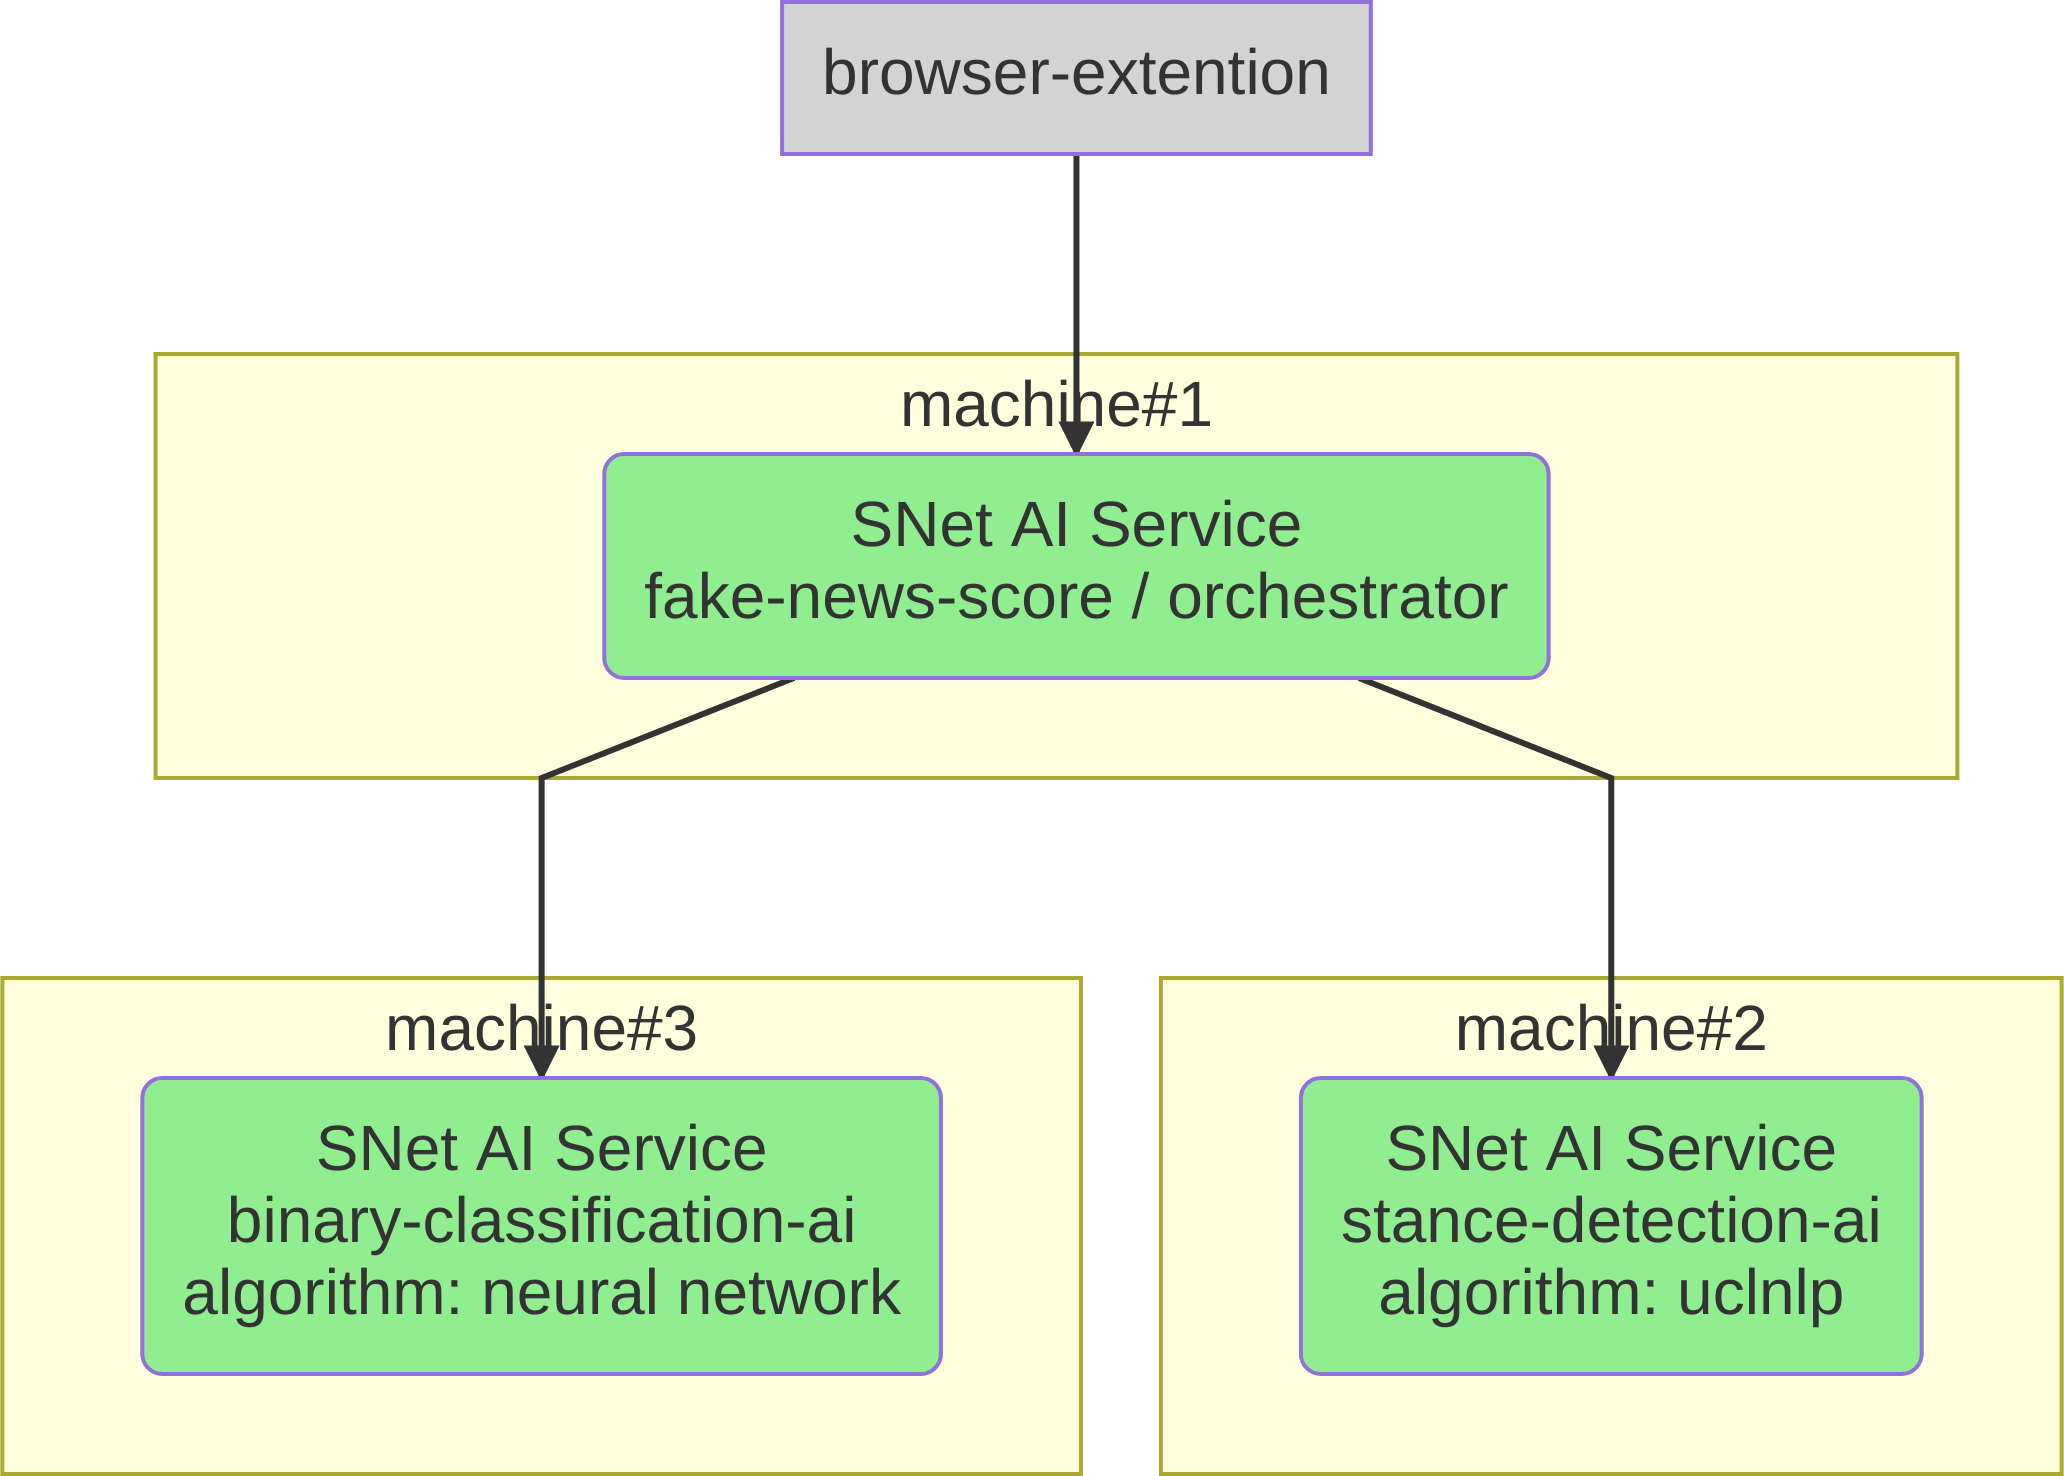
\includegraphics[width=0.9\textwidth]{../../../ontology/images/fake_news_detector.png}
    \captionsetup{width=0.8\linewidth}
    \caption{Schema of dependencies between backend components of the application
    (SingularityNET AI services potentially running on different machines).}
    \label{fig:fake_news_detector_schema}
  \end{subfigure}
  \begin{subfigure}[t]{0.50\textwidth}
    \centering
    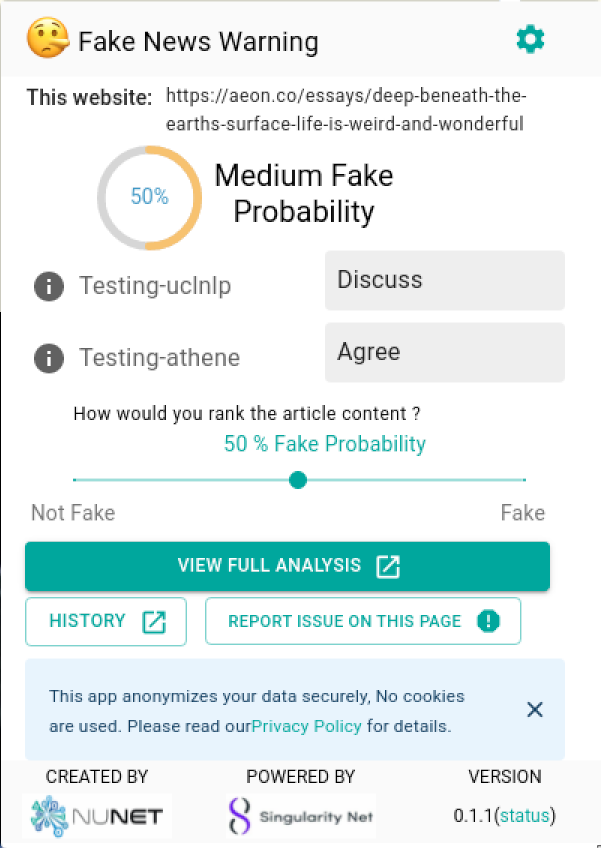
\includegraphics[width=0.5\textwidth]{../../../ontology/images/fake_news_detector_browser_extension.png}
    \captionsetup{width=0.8\linewidth}
    \caption{Brave browser extension which calls the backend of
    \texttt{Fake News Warning} application on each invocation on new
    content displayed in browser tab.}
  \end{subfigure}
\end{figure}

We will use this application design principles as the domain model for the first
design of the AI-DSL Ontology and its prototype.

\subsection{Ontology language and upper level ontology}

After discussing several choices of ontology languages and reusing existing
ontologies for designing AI-DSL ontology\footnote{See
\href{https://github.com/singnet/ai-dsl/discussions/18}{Reusing Existing
Ontologies} discussion on AI-DSL Github repository\cite{AIDSLRepo}}, we have opted to
use SUO-KIF as an ontology language~\cite{pease_standard_2009} and SUMO as an
upper-level ontology~\cite{NilesPease2001}. The main motivation for this choice
were the versatility of KIF/SUO-KIF (Knowledge Interchange Format) language,
which essentially allows to express First Order Logic (FOL) statements in a simple
text format in terms of lisp-like syntax. Due to that, KIF can be easily
converted to other formats\cite{kalibatiene_survey_2011}. Also, a conversion to
Atomese -- the OpenCog's language also employing a lisp-like syntax -- has been
successfully attempted in the past\footnote{See
the \href{https://github.com/opencog/external-tools/tree/master/SUMO_importer}{SUMO
  Importer} in the OpenCog External Tools
repository\cite{ExternalToolsRepo}}. SUMO and the related ontology design tools
\cite{pease_sigma_2001} provide a convenient way for starting to design AI-DSL
Ontology levels and their relations.

\subsection{Tools}

For the purposes of design, inital validation and displaying relations between
classes, subclasses and instances of the ontology, we have used software tools
which come together with SUMO ontology
\footnote{\href{https://ontologyportal.org}{https://ontologyportal.org}}:
\begin{itemize}
\item Sigma IDE for SUMO\footnote{\href{https://github.com/ontologyportal/sigmakee}
{https://github.com/ontologyportal/sigmakee}} and
\item jEdit plugin for SUMO
\footnote{\href{https://github.com/ontologyportal/SUMOjEdit}
{https://github.com/ontologyportal/SUMOjEdit}}
\end{itemize}

The ontology prototype, presented here, is fully accessible for browsing and
partial validation via the local Sigma installation\footnote{Can be temporarily
accessed at \href{http://nunetio.ddns.net:8080/sigma/KBs.jsp}
{http://nunetio.ddns.net:8080/sigma/KBs.jsp} or installed and accessed locally
by folowing \href{https://github.com/nunet-io/ai-dsl/blob/master/ontology/tools/README.md}{these} instructions}.

\section{Objectives and achievements}

\subsection{Decentralized ontology}

In order to satisfy the \textit{extendibility} requirement of ontology design,
we are proposing a notion and design of a \textit{decentralized ontology}, which
enables us to work with globally consistent and locally inconsistent components
within the same mechanism of AI-DSL. Based on our design, the full ontology of
\texttt{Fake News Warning} application is constructed from a number of separate
components, which operate at different level of decentralization. Table below
describes each of these components.

\begin{table}[H]
%describe each kif file / level of ontology / consistent / inconsistent;
  \scriptsize
  \centering
  \begin{tabular}{p{0.24\linewidth}|p{0.24\linewidth}|p{0.24\linewidth}|p{0.24\linewidth}|}
    \textbf{Component} &
    \textbf{Description} &
    \textbf{Dependencies} &
    \textbf{Extendability}\\
    \hline
    \href{https://github.com/ontologyportal/sumo/blob/master/Merge.kif}{Merge.kif} &
    SUMO structural ontology, base ontology, numerical functions, set/class theory, temporal concepts and mereotopology &
    None - root ontology &
    Centralized and globally enforced -- defined by \href{http://www.ontologyportal.org/}{ontologyportal.org} \\
    \hline
    \href{https://github.com/singnet/ai-dsl/blob/master/ontology/
    SingulairtyNet.kif}{SingularityNet.kif} &
    Defines global classes and types to be used for describing each
    SingularityNET AI Service &
    ComputerInput.kif, Merge.kif [,..]&
    Limited: versioning mechanism controlled by SingularityNET (to be defined)\\
    \hline
    \href{https://github.com/singnet/ai-dsl/blob/master/ontology/
    FakeNewsScore.kif}{FakeNewsScore.kif} &
    SingularityNET service responsible for constructing the whole back-end of
    each \texttt{Fake News Warning} application instance i.e. program graph
    (DAG) of the application.&
    SingularityNET.kif [,..] &
    Fully decentralized: defined by application developers; Since \texttt{Fake News
Warning} application is open source, any developer can fork it and define it
otherwise; Technically, this would be a different application.\\
    \hline
    \href{https://github.com/singnet/ai-dsl/blob/master/ontology/fnsBinaryClassifier.kif}{fnsBinaryClassifier.kif} &
    A pre-trained binary classification model for fake news detection &
    SingularityNET.kif [,..] &
    Fully decentralized: defined by each algorithm developer independently.
    Technically, from the platform perspective, these will be different
    algorithms. \\
    \hline
    \href{https://github.com/singnet/ai-dsl/blob/master/ontology/
    uclnlp.kif}{uclnlp.kif} &
    Forked and adapted component of stance detection algorithm by UCL Machine Reading group &
    SingularityNET.kif [,..] &
    Fully decentralized: defined by each algorithm developer independently.
    Technically, from the platform perspective, these will be different
    algorithms \\
    \hline
    \href{https://github.com/singnet/ai-dsl/blob/master/ontology/
    NuNetEnabledComputer.kif}{NuNetEnabledCompu-ter.kif} &
    Each NuNet enabled hardware resource will have to be described accordingly
    when on-boarded to NuNet platform &
    NuNet.kif &
    Fully decentralized: independently defined by the owner of a hardware
    resource \\
    \hline
    \href{https://github.com/singnet/ai-dsl/blob/master/ontology/NuNet.kif}{NuNet.kif} &
    Defines classes to be used for describing each hardware resource eligible
    for running SingularityNET AI Services via NuNet platform;  &
    Merge.kif, SingularityNET.kif [,..]&
    Limited: versioning mechanism controlled by NuNet (to be defined) \\
    \end{tabular}
  \captionsetup{width=0.7\linewidth}
  \caption{\label{tbl:all_kif_files}Description of each component of the AI-DSL Ontology prototype and links to related KIF files.}
\end{table}

\subsection{Ontology prototype}
\label{sec:ontology_prototype}
Using the ontology levels described in Table \ref{tbl:all_kif_files} and
referenced files, we prototyped the ontology of \texttt{Fake News Warning}
application\footnote{Can be temporarily
accessed at \href{http://nunetio.ddns.net:8080/sigma/KBs.jsp}
{http://nunetio.ddns.net:8080/sigma/KBs.jsp} or installed and accessed locally
by folowing \href{https://github.com/nunet-io/ai-dsl/blob/master/ontology/tools/README.md}{these} instructions}.

\begin{table}[H]
  \scriptsize
  \centering
  \begin{tabular}{p{0.5\linewidth}|p{0.4\linewidth}|}
    \textbf{Architectural level} & \textbf{Class} \\
    \hline
    SingularityNET platform & SNetAIService, SNetAIServiceIO,
    SNetAIServiceMetadata\\
    \hline
    NuNet platform & NuNetEnabledSNetAIService, NuNetEnabledComputer\\
  \end{tabular}
  \captionsetup{width=0.9\linewidth}
  \caption{\label{tbl:custom_classes_prototype}Main classes defined in AI-DSL
  ontology prototype per level of the \texttt{Fake News Warning} application's
  stack. Classes defined in SUMO are not included.}
\end{table}

AI algorithms onboarded on the SNet platfrom are instances of
\texttt{SNetAIService} class of sublasses of it.
Services of \texttt{Fake News Warning} application are defined as follows:

\begin{figure}[H]
  \begin{subfigure}[b]{1\textwidth}
    \centering
    \inputminted[firstline=1, lastline=2, linenos,tabsize=2,breaklines, fontsize=\small]{scm}{../../../ontology/uclnlp.kif}
    \vspace{-0.3cm}
    \captionsetup{width=0.8\linewidth}
    \caption{Service description}
    \vspace{0.3cm}
  \end{subfigure}
  \begin{subfigure}[b]{1\textwidth}
    \centering
    \inputminted[firstline=4, lastline=8, linenos,tabsize=2,breaklines, fontsize=\small]{scm}{../../../ontology/uclnlp.kif}
    \vspace{-0.3cm}
    \captionsetup{width=0.8\linewidth}
    \caption{Descriptions of service input and output types.}
    \vspace{0.3cm}
  \end{subfigure}
  \begin{subfigure}[b]{1\textwidth}
    \centering
    \inputminted[firstline=10, lastline=26, linenos,tabsize=2,breaklines, fontsize=\small]{scm}{../../../ontology/uclnlp.kif}
    \vspace{-0.3cm}
    \captionsetup{width=0.8\linewidth}
    \caption{Definition of types and their dependencies.}
  \end{subfigure}
\caption{\label{fig:serviceDefinitionKif}SNet AI Service definition in KIF
(uclnlp and binary-classification services are described in this way).}
\end{figure}

Type definitions and their dependency definitions are actually the domain of
formal type-checking part of AI-DSL and Idris related research. However,
irrespectively of which language will be eventually chosen for AI-DSL, Figure
\ref{fig:serviceDefinitionKif} expresses that we can:
\begin{enumerate}
  \item define correct serviceInput and serviceOutput types (unique for each
  service);
  \item potentially provide proofs that if a service data of correct type is
  provided on input, then it will output correctly typed data;
  \item if the above is not possible (which may be the default option when actual
  service AI are not written in Idris):
  \begin{enumerate}
    \item check if input data is of correct type at run-time and refuse to start
    service if it is not;
    \item check if output data is of correct type before sending it to the
    caller and raise error if it is not so;
  \end{enumerate}
\end{enumerate}

\texttt{FakeNewsScore} AI Service is special in that it calls
other dependent services (as described by program graph in Figure
\ref{fig:fake_news_detector_schema}) and combines their results.
We can define the program graph in
terms of dependencies between services in KIF as follows:

\begin{figure}[H]
  \captionsetup{width=0.8\linewidth}
  \inputminted[firstline=1, lastline=9, linenos,tabsize=2,breaklines, fontsize=\small]{scm}{../../../ontology/FakeNewsScore.kif}
  \vspace{-0.3cm}
  \caption{\label{fig:serviceDependencies}Defining program graph as a formal ontology. This is similar to DAG of Figure \ref{lst:dag}.}
\end{figure}

Figure \ref{fig:serviceDependencies} demonstrates how a workflow of connected
SingularityNET AI services can be statically defined and proven to work at
compile time. However, we could go further and define dependencies as
\textit{subclasses} of services with the same input/output data types. In such case
any instantiation of the subclass would be able to dynamically compile into the
workflow. Therefore we would not need to describe concrete dependencies -- they
would be dynamically resolved at run-time by matching input and output types.

\begin{figure}[H]
  \captionsetup{width=0.8\linewidth}
  \inputminted[firstline=1, lastline=22, linenos,tabsize=2,breaklines, fontsize=\small]{scm}{../../../ontology/FakeNewsScoreDynamic.kif}
  \vspace{-0.3cm}
  \caption{\label{fig:fakeNewsScoreDynamic}Defining generic input types instead
  of concrete dependencies in a \texttt{FakeNewsScoreDynamic} service.}
\end{figure}

Any AI service with output type matching input type of the
\texttt{FakeNewsScoreDynamic} could be compiled into the workflow:

\begin{figure}[H]
  \captionsetup{width=0.8\linewidth}
  \inputminted[firstline=1, lastline=4, linenos,tabsize=2,breaklines, fontsize=\small]{scm}{../../../ontology/uclnlpDynamic.kif}
  \vspace{-0.3cm}
  \caption{\label{fig:uclnlpDynamicOne}Using static globally defined types of
  input and output data structures of matching services eligible for
  compilation into a workfow.}
\end{figure}

However, systems with dependent typing, like Idris, may allow to go even further
and to find out if composite types are composed of the same components and
primitive types -- and thus match them.

\begin{figure}[H]
  \captionsetup{width=0.8\linewidth}
  \inputminted[firstline=7, lastline=26, linenos,tabsize=2,breaklines, fontsize=\small]{scm}{../../../ontology/uclnlpDynamic.kif}
  \vspace{-0.3cm}
  \caption{\label{fig:uclnlpDynamicTwo}Hypothetical usage of dynamic typing
  (most probably could be achieved in Idris, but not in KIF).}
\end{figure}

Primitive (or grounded) types (like \texttt{RealNumeber} and \texttt{Text} in
Figure \ref{fig:uclnlpDynamicTwo}), however, should be globally accessible and
unambiguously defined for this scheme to work.

All services of \texttt{Fake News Warning} application are instances of
\texttt{NuNetEnablesSNetAIService} subclass, which, in turn, is a subclass of
\texttt{SNetAIService} class:
\begin{figure}[H]
  \begin{subfigure}[t]{1\textwidth}
    \centering
    \begin{minted}[linenos,tabsize=2,breaklines,fontsize=\small]{scm}
(instance fakeNewsScore NuNetEnabledSNetAIService)
(instance uclnlp NuNetEnabledSNetAIService)
    \end{minted}
    \vspace{-0.3cm}
    \captionsetup{width=0.8\linewidth}
    \caption{Declaration of \texttt{FakeNewsScore} service in
    \href{https://github.com/singnet/ai-dsl/blob/master/ontology/
    FakeNewsScore.kif}{FakeNewsScore.kif} and of \texttt{uclnlp} service
    in \href{https://github.com/singnet/ai-dsl/blob/master/ontology/uclnlp.kif}{uclnlp.kif}.}
    \vspace{0.3cm}
  \end{subfigure}
  \begin{subfigure}[t]{1\textwidth}
    \centering
    \inputminted[firstline=1, lastline=2, linenos,tabsize=2,breaklines, fontsize=\small]{scm}{../../../ontology/NuNet.kif}
    \vspace{-0.3cm}
    \captionsetup{width=0.8\linewidth}
    \caption{Definition of \texttt{NuNetEnabledSNetAIService} in \href{https://github.com/singnet/ai-dsl/blob/master/ontology/NuNet.kif}{NuNet.kif}.}
  \end{subfigure}
  \captionsetup{width=0.9\linewidth}
  \caption{Relation between SingularityNet and NuNet domain ontologies.}
  \label{fig:SNET_and_NuNet}
\end{figure}

Figure \ref{fig:SNET_and_NuNet} describes relation between
SingularityNET and NuNet platforms. \texttt{SNetAIService} class, defined in
 \href{https://github.com/singnet/ai-dsl/blob/master/ontology/
SingularityNET.kif}{SingularityNET.kif}, contains all requirements for the
metadata of the service to be published on SingularityNET platform.
\texttt{NuNetEnabledSNetAIService} extends \texttt{SNetAIService} by adding
metadata that is needed for this service to be deployed via NuNet APIs:

\begin{figure}[H]
  \centering
  \inputminted[firstline=4, lastline=11, linenos,tabsize=2,breaklines,
  fontsize=\small]{scm}{../../../ontology/NuNet.kif}
  \captionsetup{width=1\linewidth}
  \vspace{-0.3cm}
  \caption{The definition of \texttt{NuNetEnabledSNetAIService} in
  \href{https://github.com/singnet/ai-dsl/blob/master/ontology/NuNet.kif}{NuNet.kif}
  requires a service to have compute resource (and possibly other) requirements
  included in service metadata. The idea is that without required metadata
  fields, a service would not pass validation allowing it to be deployed via
  NuNet. An arbitrary amount of requirements could be defined here.}
  \label{fig:NuNetEnabledAIService_metadata_requirements}
\end{figure}

\texttt{NuNetEnabledSNetAIService}s can be deployed only on
\texttt{NuNetEnabledComputer}s, which expose their available computing resources
in a manner that the ability to run a service is automatically checked
\textbf{before} a service is dynamically deployed on a computer and a service
call is actually issued to it (see Figure
\ref{fig:NuNetEnabledComputer_requirements}). This formally described relation
between SingularityNET and NuNet ontologies enables to prove at 'compile time'
that a service will have enough computational  resources to be executed. Recall,
that SingularityNET ontology alone enables to  prove that a service or a
collection of services will return correct results when  called with correct
inputs.

\begin{figure}[H]
  \centering
  \inputminted[firstline=13, lastline=31, linenos,tabsize=2,breaklines,
  fontsize=\small]{scm}{../../../ontology/NuNet.kif}
  \captionsetup{width=1\linewidth}
  \vspace{-0.3cm}
  \caption{The definition of \texttt{NuNetEnabledComputer} in
  \href{https://github.com/singnet/ai-dsl/blob/master/ontology/NuNet.kif}{NuNet.kif}
  requires available computing resources, computer type and operating system to
  be listed in the metadata.}
  \label{fig:NuNetEnabledComputer_requirements}
\end{figure}

An \texttt{SNetAIService} can only be deployed on \texttt{NuNetEnabledComputer}
if available resources on the computer are not less than compute requirements of
a service:

\begin{figure}[H]
  \centering
  \inputminted[firstline=38, lastline=47, linenos,tabsize=2,breaklines,
  fontsize=\small]{scm}{../../../ontology/NuNet.kif}
  \captionsetup{width=1\linewidth}
  \vspace{-0.3cm}
  \caption{Constraints on eligible match between \texttt{SNetAIService} and
  \texttt{NuNetEnabledComputer} defined in
  \href{https://github.com/singnet/ai-dsl/blob/master/ontology/NuNet.kif}{NuNet.kif}
  and required for deployment of a service.}
  \label{fig:service_deployment_requirements}
\end{figure}

\texttt{SNetAIService} and \texttt{NuNetEnabledSNetAIService} classes are positioned within the SUMO ontology as follows:

\begin{table}[H]
  \scriptsize
  \centering
  \begin{tabular}{p{0.2\linewidth}|p{0.7\linewidth}|p{0.1\linewidth}|}
    \textbf{Class, subclass or instance} &
    \textbf{Description} &
    \textbf{Where defined} \\
    \hline
    Entity &
    The universal class of individuals. This is the root node of the ontology. &
    \href{https://github.com/ontologyportal/sumo/blob/master/Merge.kif}{Merge.kif}\\
    \hline
    Abstract &
    Properties or qualities as distinguished from any particular embodiment of
    the properties/ qualities in a physical medium. Instances of Abstract can be
    said to exist in the same sense as mathematical objects such as sets and
    relations, but they cannot exist at a particular place and time without some
    physical encoding or embodiment. &
    \href{https://github.com/ontologyportal/sumo/blob/master/Merge.kif}{Merge.kif}\\
    \hline
    Proposition &
    Propositions are Abstract entities that express a complete thought or a set of
such thoughts. Note that propositions are not restricted to the content
expressed by individual sentences of a Language. They may encompass the content
expressed by theories, books, and even whole libraries. A Proposition is a piece
of information, e.g. that the cat is on the mat, but a ContentBearingObject is
an Object that represents this information. A Proposition is an abstraction that
may have multiple representations: strings, sounds, icons, etc. For example, the
Proposition that the cat is on the mat is represented here as a string of
graphical characters displayed on a monitor and/ or printed on paper, but it can
be represented by a sequence of sounds or by some non-latin alphabet or by some
cryptographic form. &
    \href{https://github.com/ontologyportal/sumo/blob/master/Merge.kif}{Merge.kif}\\
    \hline
    Procedure &
    A sequence-dependent specification. Some examples are ComputerPrograms,
finite-state machines, cooking recipes, musical scores, conference schedules,
driving directions, and the scripts of plays and movies. &
    \href{https://github.com/ontologyportal/sumo/blob/master/Merge.kif}{Merge.kif}\\
    \hline
    ComputerProgram &
    A set of instructions in a computer programming language that can be
    executed by a computer. &
    \href{https://github.com/ontologyportal/sumo/blob/master/Merge.kif}{Merge.kif}\\
    \hline
    SoftwareContainer &
    &
    \href{https://github.com/singnet/ai-dsl/blob/master/ontology/
    SingulairtyNet.kif}{Singularity-Net.kif}\\
    \hline
    SNetAIService &
    Software package exposed via SNetPlatfrom and conforming to the special
    packaging rules &
    \href{https://github.com/singnet/ai-dsl/blob/master/ontology/    SingulairtyNet.kif}{Singularity-Net.kif}\\
    \hline
    NuNetEnabled-SNetAIService &
    SNetAIService which can be deployed on NuNetEnabledComputers and
    orchestrated via NuNet platfrom &
    \href{https://github.com/singnet/ai-dsl/blob/master/ontology/    NuNet.kif}{NuNet.kif}\\
    \hline
    \quad \texttt{uclnlp} &
    Forked and adapted component of stance detection algorithm by UCL Machine
    Reading group. &
    \href{https://github.com/singnet/ai-dsl/blob/master/ontology/    uclnp.kif}{uclnlp.kif}
  \end{tabular}
\captionsetup{width=0.9\linewidth}
\caption{\label{tbl:uclnlp_hierarchy}Full hierarchy of dependencies of
\texttt{uclnlp} SNet AI service instance within SUMO ontology. The same
hierarchy applies to \texttt{binary-detection} and \texttt{fakeNewsScore} services used
in the \texttt{Fake News Warning} app.}
\end{table}

\subsection{The mechanism of dynamic workflow construction}

An important part of the \textit{decentralized ontology} design is the mechanism
which makes it work in actual scenarios. This mechanism was designed using the
same domain model of \texttt{Fake News Warning} application. It also clarifies
the reason why we propose this particular concept and design of
\textit{decentralized ontology}.

AI-DSL will allow to search, match, compile and
execute independently developed AI components in terms of a single veritable
workflow running on SingularityNET platform. AI components of the workflow may
be developed using different programming languages by different people, 
have different licenses and, actually, may be developed with different initial
goals. Furthermore, these workflows will be executed on the machines owned by 
different entities. In a decentralized system like this, each developer will be
able to freely choose properties, capabilities and internal structure of their
algorithms. Through the mechanism of dynamic workflow construction, AI-DSL will
be able to pull together the information about each component of desired workflow
when the execution of it is required.

The very high level view of SingularityNET's
AI Service calls involving AI-DSL looks as follows:

\begin{figure}[H]
	\centering
	\includegraphics[width=0.9\textwidth]{../../../ontology/images/high-level-workflow-construction.png}
	\captionsetup{width=0.9\linewidth}
	\caption{\label{fig:high-level-workflow-construction}Bird's eye view of 
		application-independent SingularityNET calls involving AI-DSL.}
\end{figure}

Within the domain model of \texttt{Fake News Warning} application (Figure 
\ref{fig:fake_news_detector_schema}) this scheme works approximately in the following
way:
\begin{enumerate}
\item \textit{User/Business} accesses the platform 
via browser-extension by sending (a) the definition of the workflow to the
platform in the form of a DAG (Figure \ref{lst:dag}) and 
(b) the web content to be checked for probability to contain fake news.
\item The AI-DSL engine reads the DAG and identifies the dependent SNet AI Services that
need to be called.
\item If dependent services are indicated statically as in \ref{lst:dag},
then the platform knows immediately names of the services to be called. If, however,
dependent services are described in terms of their input / output types (as in
\ref{fig:serviceDependencies}), the AI-DSL engine searches and matches services available
in the platform that satisfy constraints defined there\footnote{In the
future, the AI-DSL engine
will aim to accommodate fuzzy service definitions and complex decision functions to
search and match them, involving ability for an AI Service to choose its
dependent services.}.
\item When matching services are found, the AI-DSL engine pulls their individual type
signatures and other metadata from each service (note, that a decentralized system
cannot be built with the assumption of availability of global registry; such registry
can, however, be built as a secondary index of otherwise decentralized information
sources) and compiles into a workflow. This operation may be done in a few stages:
\begin{itemize}
	\item When the AI-DSL engine requests metadata for the dependent service and receives it,
	it checks the received metadata for conformance to AI-DSL Ontology requirements
	(e.g. well-formed description in SUO-KIF and correct type dependencies as defined
	hierarchy in Table \ref{tbl:uclnlp_hierarchy} and displayed graphically in
	Figure \ref{fig:uclnlp_hierarchy_graph}):
	
\begin{figure}[H]
	\centering
	\includegraphics[width=1\textwidth]{../../../ontology/images/uclnp_hierarchy_graph.png}
	\captionsetup{width=0.9\linewidth}
	\caption{\label{fig:uclnlp_hierarchy_graph}Graphical form of the hierarchy of 
	dependencies of \texttt{uclnlp} SNet AI service instance of \texttt{Fake News Warning} 
	application within SUMO ontology.}
\end{figure}

\pgfkeys{/csteps/inner color=white}
\pgfkeys{/csteps/outer color=black}
\pgfkeys{/csteps/fill color=black}

	\item Note, that the correctness of type dependencies of decentralized components of 
	the AI-DSL Ontology (\texttt{uclnlp}) will be checked against centralized
	components versioned by SingularityNET platform (Table \ref{tbl:all_kif_files}). Defining
	versioning mechanism of global components of the ontology is not within the scope 
	of this work. However, merely acknowledging the possible existence of different 
	versions of root and middle level ontologies within the hierarchy requires to 
	think about reasonable way to accommodate them into the system. A possibility 
	is to include information about the version of global components of ontology when 
	communicating decentralized components between each other, 
	as suggested in \cite{YvesHellenschmidt2002}. 
	In such case, the stage \Circled{4} of the workflow construction 
	in Figure \ref{fig:high-level-workflow-construction} would look approximately like this:
	
\begin{figure}[H]
	\centering
	\includegraphics[width=1\textwidth]{../../../ontology/images/verification_for_workflow_correctness.png}
	\captionsetup{width=0.9\linewidth}
	\caption{\label{fig:verification-sequence}Stage \Circled{4} of workflow construction 
		sequence (fully depicted in Figure \ref{fig:high-level-workflow-construction}) -- compiling the workflow and
		proving its correctness.}
\end{figure}

	\item Service metadata returned by calls \Circled{2} and
          \Circled{4} of Figure \ref{fig:verification-sequence} include service definitions
	and the version number of the global AI-DSL Ontology that was used to build these definitions. For
	example, call \Circled{4} may contain the following information:

	\begin{figure}[h]
		\centering
		\begin{minted}[linenos,tabsize=2,breaklines, fontsize=\small]{json}
		{
			"sender": "uclnlp",
			"receiver": "fakeNewsScore",
			"upper-ai-dsl-ontology": "v0.1",
			"service-metadata": $(include sevice_definition.json),
			"leaf-ontology": $(include uclnlp.kif)
		}
		\end{minted}
		\vspace{-0.3cm}
		\captionsetup{width=0.8\linewidth}
		\caption{\label{lst:uclnlp_metadata}Metadata of the \texttt{uclnlp} service. Sample contents 
			of included files can be seen separately for each  
			\href{https://gitlab.com/nunet/fake-news-detection/uclnlp/-/blob/master/service/service_spec/service_definition_prod.json}{service\_definition.json}
			and \href{https://github.com/singnet/ai-dsl/blob/master/ontology/uclnlp.kif}{uclnlp.kif}.
		}
	\end{figure}

	\item When all service definitions are collected and the their versions checked to match, 
	they can be checked for conformance with the global AI-DSL Ontology of respective version and,
	if service definitions include type signature -- type-checked.
	
	\item The actual compilation of the workflow, compliance to
          the AI-DSL Ontology and type-checking need a
	dedicated and properly configured execution environment. In the context of this document, 
	that execution environment may include the Idris compiler, an ontology prover that is able to process 
	SUO-KIF definitions (e.g. Sigma), their dependencies and possibly custom code.
	For that, it would be most logical to introduce a dedicated
	AI service into the platform -- which is the \texttt{verifier} component denoted in Figure 
	\ref{fig:verification-sequence}. The \texttt{verifier} service will be able to run any required
	verification procedures in order to provide a proof that the workflow constructed from 
	services found in step \Circled{3} is valid and can be correctly executed on the 
	SingularityNET platform.

	\item After calls \Circled{1}, \Circled{2}, \Circled{3} and \Circled{4} of 
	Figure \ref{fig:verification-sequence} are completed, a call \Circled{5} will be issued to
	 \texttt{verifier} sending all metadata of each  service along
	 with the AI-DSL Ontology version's identifier. The \texttt{verifier} will then 
	 request all required dependencies
	 (listed in Figure \ref{tbl:all_kif_files}) from the central SingularityNET repository 
	 (or blockchain) and calculate the proof.
	\item After \texttt{verifier} calculates the proof at step \Circled{8}, 
	the proof is sent to the service that has requested it (in the case of
	\ref{fig:high-level-workflow-construction} -- to \texttt{fakeNewsScore}). 
	Additionally, the existence of independent verifiers would allow to optimize the overall computational 
	costs of calculating proofs on the platform, by recording them into the blokchain and making
	 searchable by other services that may require the same workflow. One way to do this would be to:
	\begin{enumerate}
		\item Calculate a hash from the metadata of each service of the workflow 
		(i.e. *.kif or *.idr files);
		\item Construct a Merkle tree
		\footnote{\href{https://en.wikipedia.org/wiki/Merkle_tree}{https://en.wikipedia.org/wiki/Merkle\_tree}} 
		from those hashes which would exactly mirror the structure of the workflow 
		defined in DAG (Figure \ref{lst:dag});
		\item Record the root hash of the tree into the blockchain with relevant metadata;
	\end{enumerate}

	 \item Such setup would constitute an implicit reputation system of workflows in the sense that
	 a workflow with most proofs of correctness on the blockchain could be trusted to work without
	 recalculating the proof each time a workflow is constructed.

\end{itemize}

\end{enumerate}

\section{Future work}

\begin{itemize}
  \item In the long term, it may be ideal to develop a converter for converting
OWL to KIF, since OWL may be representable in KIF
\cite{martin_translations_nodate}  using \href{https://github.com/owlcs/owlapi}{OWL
	API}; For the purpose of the ontology
prototype, we are manually selecting parts of the existing ontologies in order to build
the prototype and write them in SUO-KIF format.
  \item Similarly we want to be able to convert SUO-KIF specifications
    into Idris, and possibly vise versa, to take advantage of the strengths of
    each formalism.  To the best of our knowledge there are no existing
    tools to automatically translate SUO-KIF to/from Idris, however
    there is a tool to translate SUO-KIF to
    FOL~\cite{Pease_firstorder} and a paper describing
    the translation from a Dependently Typed Language (DTL) to
    FOL~\cite{SojakovaKristina2009}.  Additionally, to start building
    an understanding about such process, we have manually ported the trivial AI
    services described in Section \ref{sec:dependently_typed_registry} to SUO-KIF, see
    \href{https://github.com/singnet/ai-dsl/blob/master/ontology/TrivialServices.kif}{TrivialServices.kif}
    under the
    \href{https://github.com/singnet/ai-dsl/blob/master/ontology}{ontology}
    of the \href{https://github.com/singnet/ai-dsl/}{AI-DSL
      repository}~\cite{AIDSLRepo}.  As it turns out writing formal
    specifications of functions in SUO-KIF is reasonably straight
    forward.  Here is for instance the SUO-KIF implementation of the Twicer service
\begin{minted}[mathescape]{idris}
(instance TwicerFn UnaryFunction)
(domain TwicerFn 1 Integer)
(range TwicerFn EvenInteger)
(=>
  (instance ?INTEGER Integer)
  (equal (TwicerFn ?INTEGER) (MultiplicationFn ?INTEGER 2))))
\end{minted}
where \texttt{EvenInteger} happens to be predefined in
\href{https://github.com/ontologyportal/sumo/blob/master/Merge.kif}{Merge.kif}
of SUMO, partially recalled below
\begin{minted}[mathescape]{idris}
(=>
  (instance ?NUMBER EvenInteger)
  (equal (RemainderFn ?NUMBER 2) 0))
\end{minted}
Thus one can see that is it easy to specify a function input type,
using \texttt{domain}, and output type, using \texttt{range}, in
SUO-KIF, as well its full or partial definition, using \texttt{=>},
\texttt{equal} and universally quantified variables such as
\texttt{?NUMBER}.  It should be noted however that the reason it works
so well in that case is because the output type does not depend on the
input value, the output is an even integer no matter what.  It is
expected that porting for instance the \texttt{append} function of the
dependent type \texttt{Vect}~\cite{Vectors} to SUO-KIF might not be as
trivial, since the \texttt{domain} and \texttt{range} constructs may
not be suitable to represent such dependence (i.e. that the size of
the resulting vector of \texttt{append} is the sum of the sizes of the
input vectors).  However, given that dependent types are essentially
functions, it might be possible to set the \texttt{domain} and
\texttt{range} with such type functions.  Alternatively such
dependence can be moved to the function definition as offered by
SUO-KIF expressiveness.  Another aspect we need to explore is how
tools, such as Automatic Theorem Provers
(ATPs)~\cite{Baumgartner_automatedreasoning, Urban_anoverview,
  Alvez_evaluating_atp_adimen_SUMO}, can be used to autonomously
compose as well as retrieve functions given their input and output
types.  Obviously if ATP tools running over SUO-KIF turn out to be
deficient in that respect, we already know from Section
\ref{sec:dependently_typed_registry} that Idris can fulfill that
purpose.
\end{itemize}

\chapter{Software Engineering Strategies}
\label{chap:soft_eng_strat}
\section{Service Composition in Idris2}
\label{sec:service_composition_in_idris2}

A key requirement of the AI-DSL is to provide both an ergonomic syntax for
describing service properties and a robust process for using these descriptions
to verify the correctness of composed services.  This work involved
investigating several different methods for meeting this requirement using
Idris2.

\subsection{\texttt{RealizedFunction} and \texttt{RealizedAttributes}}
The \texttt{RealizedFunction} and \texttt{RealizedAttributes} data types were an
early strategy for describing and composing AI services.  They directly
contained values representing the relevant properties of arbitrary Idris
functions and made use of a \texttt{compose} function to compute the properties
of the function resulting from the composition of two others.

While this approach worked to verify that a small, fixed set of attributes was
correct for a composition of functions, it also presented several issues:

\begin{itemize}
  \item
        The \texttt{RealizedFunction} definition contains only the raw data
        representing function properties, while using a separate function to
        represent composition logic.  Because the composition logic is not
        part of the type definition, there is no way for Idris to prove that the
        correct logic was used to construct any given \texttt{RealizedFunction}.


  \item \texttt{RealizedAttributes} represents only a set of example properties.
        The syntax tree for the AI-DSL should be able to represent any
        properties specified by the user, assuming the composition laws for
        those properties are known.


\end{itemize}

\subsection{\texttt{Service}}
To address these problems, we implemented the \texttt{Service} type,
which can be found in
\href{https://github.com/singnet/ai-dsl/blob/master/experimental/realized-function/ServiceAttributes.idr}{\texttt{experimental/realized-function/ServiceAttributes.idr}}.
It differs from \texttt{RealizedFunction} in two important ways:
\begin{itemize}
  \item Composition logic is represented entirely at the type level as a second
        constructor for the \texttt{Service} type.

  \item Idris' \texttt{Num} interface is used as a generic representation of any
        attribute that can be added when two \texttt{Service}s are sequenced.

\end{itemize}

These changes were sufficient to solve the problems with our earlier approach,
but we still needed to improve the expressiveness of our representation.  Many
important properties are too complex to be described using only the \texttt{Num}
interface.

\subsection{A Look into Dependent Pairs}
\label{sec:dependent_pairs}
Idris represents the intersection between a theorem proof assistant and a
programming language.  As such, it is often useful to think of types as
logical propositions, and values as proofs of those propositions.  Since our
goal is to verify that a desired property is true of some value, we can use
dependent types to describe a proposition parameterized by a specific value.

Idris provides a special syntax for this.
\texttt{(x : a ** p)} can be read as ``\texttt{x} is a value of type \texttt{a} such that
proposition \texttt{p} holds true of \texttt{x}''.  This is called a dependent pair, and it can
only be constructed by providing both a value and a proof that a desired
property holds true for that specific value.  In the context of service
composition, we can use dependent pairs as a direct representation of input
values that satisfy some condition.

To demonstrate the practicality of this pairing, consider the following types:

\begin{minted}[mathescape]{idris}

public export
data WFInt : Type where
     Nat : (n : Nat) -> WFInt
     Neg : (n : Nat) -> WFInt --Note: In the negative case, n=Z represents -1.

-- n-parity, i.e. proof that an integer a is evenly divisible by n (or not).
public export
data Parity : (a : WFInt) -> (n : WFInt) -> Type where
     -- a has even n-parity if there exists an integer multiple x s.t. x*n = a.
     Even : (x : WFInt ** (x * n) = a) -> Parity a n

public export
data OddParity : (a : WFInt) -> (n : WFInt) -> Type where
     -- a has odd n-parity if there exists
     Odd : (b : WFInt ** LT = compare (mag b) (mag n))
      -> (Parity (a + b) n) ->  OddParity a n

\end{minted}

\texttt{WFInt} is a type describing a well-founded view of an integer.  This
alternate view is necessary in order to write more flexible inductive proofs for
integer inputs.

\texttt{Parity} demonstrates the proof obligation necessary to
show that one integer is evenly divisible by another.  In plain English, it can
be read as ``If there exists some integer \texttt{x} such that
\texttt{x * n = a}, then \texttt{a} can be said to have \texttt{n-parity}.''
\texttt{OddParity} is a type representing the opposite proposition, i.e. that
dividing two integers will produce a remainder.

For services such as our Halfer example, this allows us to clearly express that
inputs should be only even numbers, as shown in this function type signature:

\begin{minted}[mathescape]{idris}
halfer : (a : WFInt ** Parity a 2) -> WFInt
\end{minted}

Similarly, the type signatures of the Twicer and Incrementer example services
can express their properties with regards to the 2-parity of the integers they
operate on:

\begin{minted}[mathescape]{idris}
-- Guaranteed to produce a value divisible by 2
twicer : (b : WFInt) -> (a : WFInt ** Parity a 2)

incrementer : (a : WFInt ** Parity a n) -> (b : WFInt ** OddParity b n)
\end{minted}

Now that the relevant properties for verification are expressed entirely at the
type level, the Idris2 typechecker can statically check the validity of service
compositions.

\begin{minted}[mathescape]{idris}

-- A valid sequence of services that successfully typechecks.
compo1 : WFInt -> WFInt
compo1 = fst (incrementer . halfer . twicer)

-- An invalid sequence of services that will always fail typechecking
compo2 : WFInt -> WFInt
compo2 = fst (halfer . incrementer . twicer)
\end{minted}

With dependent pairs, arbitrary properties of values can be encoded and formally
verified.  For an AI-DSL that may need to describe AI services in many different
contexts, this ability to use custom types instead of a limited set of
primitives is crucial.  However, this method is not a complete solution, as it
highlights major practical flaws.

An AI service developer making use of the AI-DSL should be able to adequately
describe the necessary properties of data their service will take as input, but
there should be no need for them to also encode the exact properties of their
service's output data.  A service developer is not likely to have any knowledge
of how their service's outputs will be used by other services in the future, so
the AI-DSL should not force them to describe their output data in any more
detail than is possible\footnote{Of course given a full specification
of the service, which is admittedly hard but possible to provide, any
decidable correct property about its output data can be inferred,
possibly at a prohibitively high cost.}.  In the examples above,
the \texttt{incrementer} service was forced to describe its inputs and
outputs in terms of properties that are only relevant to other
services.


\subsection{A Monadic DSL}

At this stage, there are two key problems which must be solved:

\begin{enumerate}

  \item At the point of service creation, developers should not be expected to
        have knowledge of the properties that are only relevant to other
        services.  They should be able to encode only the properties relevant to
        their own service.

  \item Due to the limits of computability, some relevant properties of data
        will not be formally provable.  However, some of these properties might
        still be safely assumed to hold in certain contexts, even if a formal
        proof is impossible.  The AI-DSL should be able to represent such cases
        and provide the strongest possible guarantees.

\end{enumerate}

For the first issue, we borrowed a well-established design pattern from
strongly-typed functional programming and defined a new \texttt{Service} type
around the \texttt{Monad} interface\nil{Sam, could you add a citation
  about that ``well-established design pattern'' you are referring
  to?}\nil{Sam, could you add reference to the code in question?}.
Monads are a class of types used to
describe a context for operations, along with any custom logic necessary to
combine those operations without imposing any requirement for tight coupling.
This is perfect for the AI-DSL.

To address the issue of unproveable properties, we experimented with a
conceptual model of smart contracts as a core language feature within the DSL.
Because the actual implementation of logic to represent external smart contracts
was outside the scope of this work, we made the assumption that such contracts
could be used to represent a financially-backed assurance that some unproveable
property holds.  In theory, this could allow compositions of AI services to be
analyzed for their overall financial risk.



\section{Depth of Embedding}
\nil{Sam, can you add citations related to that Section?}
A domain-specific language requires not only a formal specification for its
semantics, but a software implementation as well.  The relationship between a
DSL and its implementation can vary, but most strategies fall into one or more
of three categories:

\begin{enumerate}
  \item \texttt{Independent Syntax:} A language may be designed completely
        separately from its implementation.  Such languages typically require
        dedicated compilers or interpreters, as they are unable to borrow any
        functionality due to their lack of a host language.

  \item \texttt{Shallow Embedding:} An embedded domain-specific language (eDSL)
        is written as a module or library for some host language.  Data in the
        DSL's domain is represented directly as values in the host language.
        Shallow embeddings tend to be easy to use and extend, but often suffer
        issues with performance and expressiveness.  Programs written in a
        shallowly-embedded DSL can only describe operations in the domain of
        their host language, and thus are limited to a single interpretation.

  \item \texttt{Deep Embedding:} Similarly to a shallowly-embedded DSL,
        an eDSL with a deep embedding is defined in some host language.
        Deep embeddings define a custom Generalized Algebraic Data Type
        (GADT) in the host language and represent
        all data as values of this type.  Because the entire Abstract Syntax
        Tree (AST) of a deeply-embedded program is a single type, it is simple to
        write functions in the host language that operate directly on the
        embedded program. This allows for automatic optimization of embedded
        programs, as well as multiple possible interpretations.  However, any
        extensions to a deep eDSL require significant effort, as changes to the
        language's AST type incur a requirement to update every function that
        operates on that type.

\end{enumerate}

For the AI-DSL, the most promising approach appears to be a hybrid method.
The basic domain of the DSL can be defined as deep embedding, while more
specialized features can be shallowly embedded as smaller DSLs within the main
AI-DSL instead of directly in Idris2.



\chapter{Conclusion (draft)}

The novel nature of such a project requires a large amount of
exploration, which is what this iteration has been all about.  From
the start we agreed that we wanted to take a holistic approach, attempting
to achieve a full albeit limited prototype as rapidly as possible in
order to uncover hidden blocks as early as possible.

With that mind let us summarize what we have accomplished so far and
what are the next steps to bring us closer to a complete AI-DSL.  We
have
\begin{itemize}
\item Experimented with Idris to formalize and reason about realized
  function attributes such as costs and quality, see Section
  \ref{sec:realized_function}.  We have done so in a limited manners, only
  considering additive cost and infimum-itive quality, but we have
  proven that it is possible and tractable to do in Idris.  More work
  is required to expand the complexity of such realized function
  attributes, such as functional or distributional costs and quality.
\item Experimented with Idris to formalize function properties as
  dependent types, see Chapter \ref{chap:soft_eng_strat}.  Again this
  was done in a limited manner, using trivial properties such as
  evenness of numbers, but taught us that it is a possible to do in
  Idris, and provided us insights on how to expand that to more
  complex properties.
\item Built a prototype of a Dependently Typed Registry to retrieve,
  match and connect AI services based on their specifications as
  dependent types, see Section \ref{sec:network_idris_ai_services}, using Idris
  meta-functions for function matching and retrieval.  This prototype
  has limits, such as returning only the first matching AI service and
  not performing fully autonomous composition of AI services, but none
  of these limits seem fundamentally hard to address and should only
  require more development time.
\item In Chapter \ref{chap:aidsl_ontology} we have explored ontologies
  with the goal of defining a rich and extendable vocabulary for
  specifying AI services, their algorithms, data types as well as
  their relationship to real world.  The decision was made to build
  such AI ontology on top of SUMO due to its openness, breadth and
  quality.  TODO: concrete extension (read Kabir's work and mention
  trivial AI services).  More work is required to TODO.  We also
  explored how to convert SUO-KIF knowledge into Idris, more work is
  required to automate such conversions.
\item Reviewed literature of related work to make sure we do not miss
  anything major and can take advantage of existing technologies.
  Even though we have found no such related project using Dependent
  Types as central component, there are related endeavors described in Section
  \ref{sec:related_work} with potential reusable ideas, languages or code,
  such as FIPA-ACL and more.  More exploration is needed on that front
  as well.
\item Experimented with various approaches for defining AI-DSL as an
  Idris eDLS, see Chapter \ref{chap:soft_eng_strat}.
\item Started building, though more at the preparatory level, a real
  world AI service assemblage test case, based on Nunet Fake News
  Warning example.  See Chapter \ref{TODO}.  Such test case is going
  to be critical to put our AI-DSL prototypes to the test and build
  the understanding necessary to push it to the next level.
\end{itemize}
The work taking place during the next iterations will consist in
continuing such exploration, refining our existing prototypes and
bringing them together in a holistic system, guided by real world AI
service assemblage test cases.  Such test case will initially include
the Nunet Fake News Warning collective.  Then more test cases will be
considered over various domains such as bio-informatics, finance,
embodied agent control and more.

To conclude, even though there is a long way to go, we believe a lot
has been accomplished already, and we are happy to say that no
profound difficulties have been revealed so far, although we must
remain cautious.  One difficulty that is expected to eventually come
up is the tractability of the verification and automated composition
process of AI services.  This is generally undecidable, and even when
restricted to subclasses of functions (as is the case in Idris due to
being based on Intuitionistic Logic) can still have explosive
complexity.  However, it is also expected that a tremendous amount of
value will be created by having such system work with restricted
applicability.  Ultimately is it expected that the AI-DSL will need to
synergies with AGI systems which, uncoincidentally, is one of the
quintessential functions that SingularityNET aims to offer.

\appendix
\chapter{Glossary}
\begin{itemize}
\item \textbf{AI service assemblage}: collection of AI services
  interacting together to fulfill a given function.  Example of such
  AI service assemblage would be the Nunet Fake News Warning system.
\item \textbf{Dependent Types}: types depending on values.  Instead of
  being limited to constants such as \texttt{Integer} or
  \texttt{String}, dependent types are essentially functions that take
  values and return types.  A dependent type is usually expressed as a
  term containing free variables.  An example of dependent type is
  \texttt{Vect n a}, representing the class of vectors containing
  \texttt{n} elements of type \texttt{a}.
\item \textbf{Dependently Typed Language}: functional programming
  language using dependent types.  Examples of such languages are
  Idris, AGDA and Coq.
\end{itemize}

\bibliographystyle{splncs04}
\bibliography{local}

\end{document}
